\section{Results}
\label{section:results}

The results section discusses the empirical analysis of the clustering methods tested during the implementation of the Ownership Assignment process. 
The experiment design is simple and designed to provide an upper bound for performance on an optimal dataset with no noise (the Swan Valley wineries dataset.) 
The Swan Valley Wineries dataset consists of 31 wineries retrieved from OSM and \~150 objects hand-labelled across 6 of those 31 locations with ground-truth location labels. 
%The objective of the experiment was to see which clustering method most accurately predicts the location that the objects 'belong' to. Here accuracy is measured in two dimensions. 
%First: the predicted location / true location label match. Second, the creation of the correct number of clusters (6).
%Testing of K-Means and DBSCAN occurs under optimal, realistic and worst-case parameter conditions. For both DBScan and K-Means, the location is inferred to be the location coordinate closest to the cluster centroid. 

%\subsection{K-Means}
%K-Means clustering accepts the input of a collection of object coordinates and a parameter $K$ of the number of clusters to create. 
%Optimal conditions assume the number of clusters is known ($K=6$). 
%Realistic conditions assume the number of clusters equals the number of locations ($K=31$), and worst-case conditions assume only one cluster ($K=1$). 

%\begin{figure*}[h]
%\centering

%\begin{subfigure}[t]{.3\textwidth}
%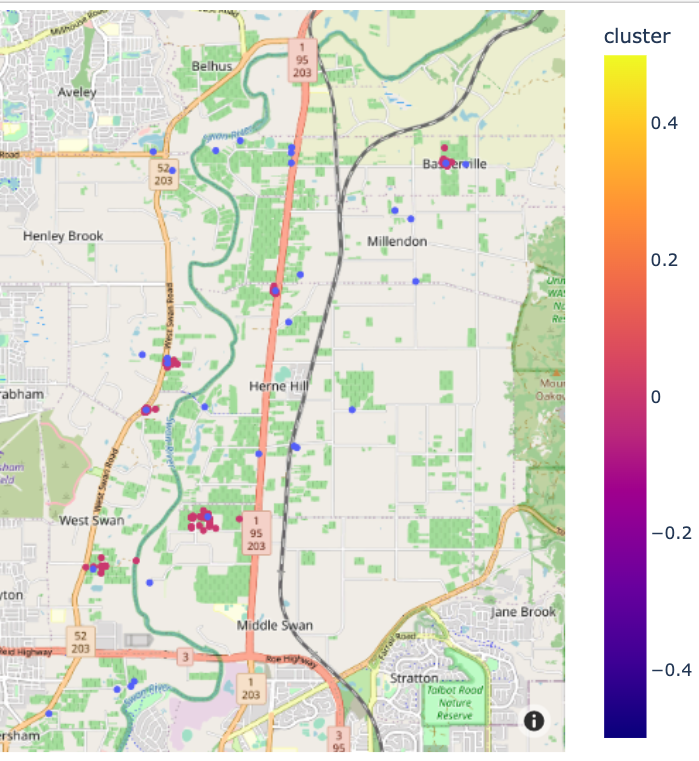
\includegraphics[width=\textwidth]{gestalt_kmeans_k1.png}
%\caption{In the worst case of $K=1$, all objects are incorrectly assigned to the central location of the region.} % 
%\label{fig:kmeans_worst}
%\end{subfigure}
%\hfill
%\begin{subfigure}[t]{.3\textwidth}
%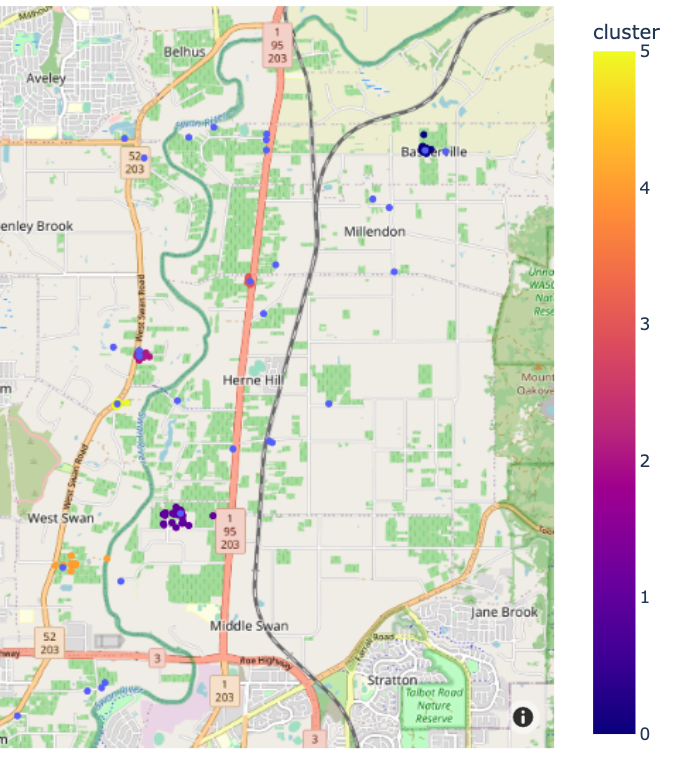
\includegraphics[width=\textwidth]{gestalt_kmeans_k6.png}
%\caption{\small With optimal conditions $K=6$, the %clustering performs ideally, while locations are sparse across the region.}
%\label{fig:kmeans_optimal}
%\end{subfigure}
%\hfill
%\begin{subfigure}[t]{.3\textwidth}
%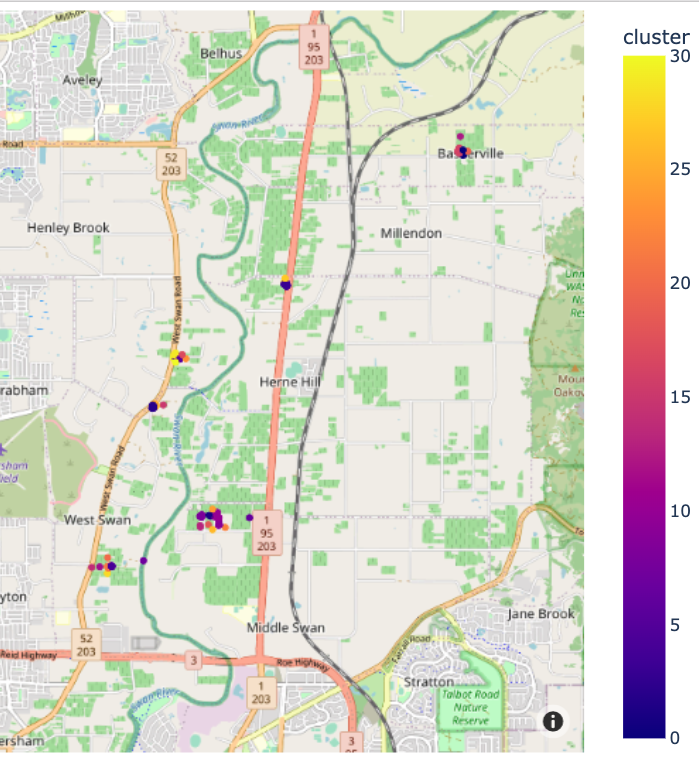
\includegraphics[width=\textwidth]{gestalt_kmeans_k31.png}
%\caption{\small In realistic settings where $K=Number of Locations$, it clusters incorrectly but assigns the correct owners, which is unlikely to hold when location density increases}
%\label{fig:kmeans_realistic}
%\hfill
%\end{subfigure}

%\caption{\textbf{K-Means Performance.} In regions with sparse locations K-Means performs well even if too many clusters exist; this is unlikely to be true in dense regions.}

%\label{fig:kmeans_experiments}
%\end{figure*}

%Unsurprisingly, the optimal situation performed best with all objects assigned to their correct clusters and all clusters assigned to their correct label. One reported misclassification was determined to be a labelling error in the training data. Surprisingly, under 'realistic' conditions, though the number of clusters is far more than there should be, it correctly assigns the ownership of almost all objects with only five incorrectly labelled. Under the worst-case conditions, it only creates a single cluster and assigns all objects to the (same) incorrect location. 

%\subsection{DBSCAN}
%The DBSCAN algorithm was introduced in 1996 by Ester et al. \cite{Ester1996}. It is a clustering algorithm that accepts the input of a collection of object coordinates and two parameters $\epsilon$, the distance permitted between coordinates before they transition to a different cluster and $N$ the number of coordinates required to be within $\epsilon$ of each other to form a cluster. 
%A 2017 paper by Schubert et al. \cite{Schubert2017} provides useful guidance on turning these parameters, and their experiments reveal that the value of $\epsilon$ is much more sensitive than the value of $N$. Based on their guidance, optimal conditions would see $\epsilon \leftarrow (2xdim)-1 = 3metres$. Their guidance further notes that domain knowledge should be used where appropriate, so here we set ($\epsilon = 10 metres$). Realistic sets ($\epsilon = 100 metres$) and worst case sets ($\epsilon = 1000 metres$). $N=3$ in all tests. 

%\begin{figure*}[h]
%\centering

%\begin{subfigure}[t]{.3\textwidth}
%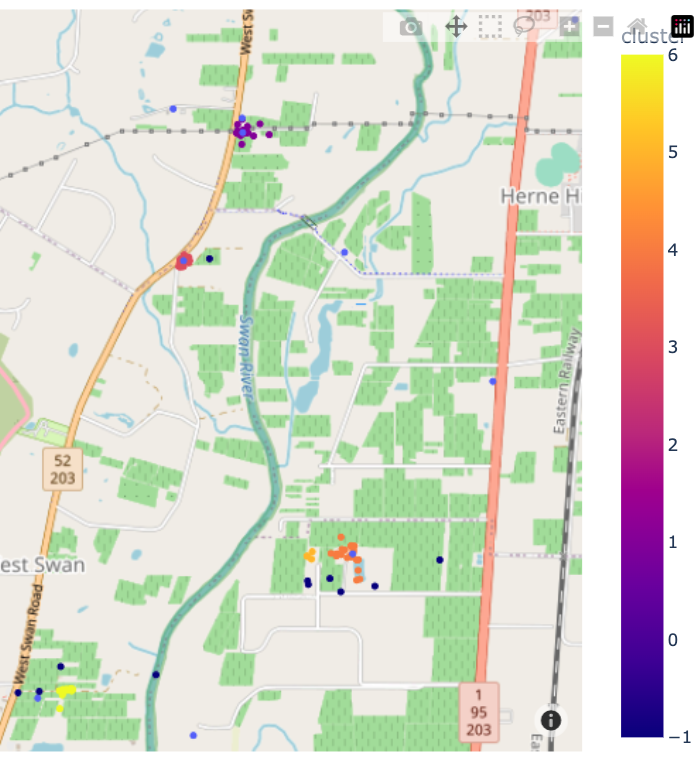
\includegraphics[width=\textwidth]{gestalt_dbscan_e10.png}
%\caption{In the optimal case of $\epsilon=10$ 12 objects are incorrectly pruned as 'noise' (cluster = -1).} % 
%\label{fig:dbscan_optimal}
%\end{subfigure}
%\hfill
%\begin{subfigure}[t]{.3\textwidth}
%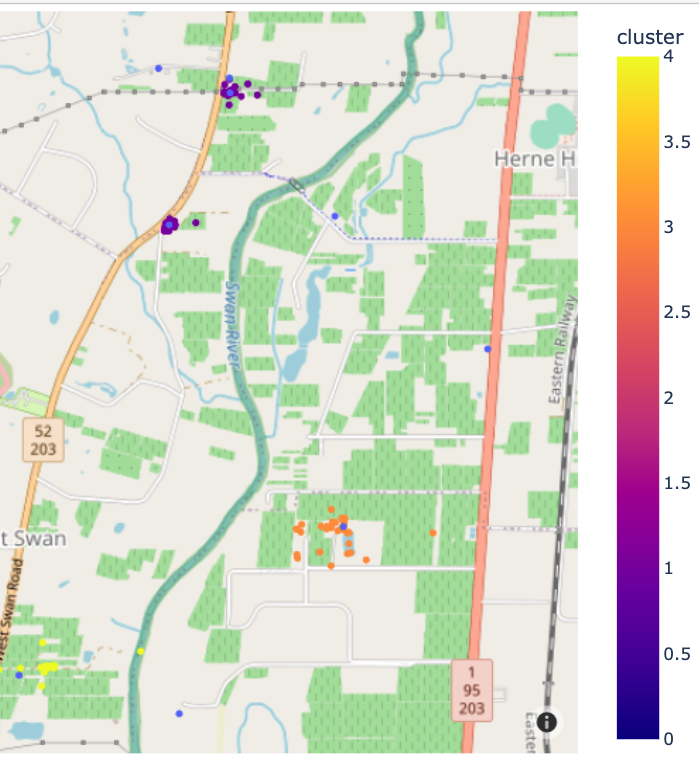
\includegraphics[width=\textwidth]{gestalt_dbscan_e100.png}
%\caption{\small With realistic conditions $\epsilon=100$ the \textit{ugly duckling wines} and \textit{Little River Winery} merge because the locations are too close.}
%\label{fig:dbscan_realistic}
%\end{subfigure}
%\hfill
%\begin{subfigure}[t]{.3\textwidth}
%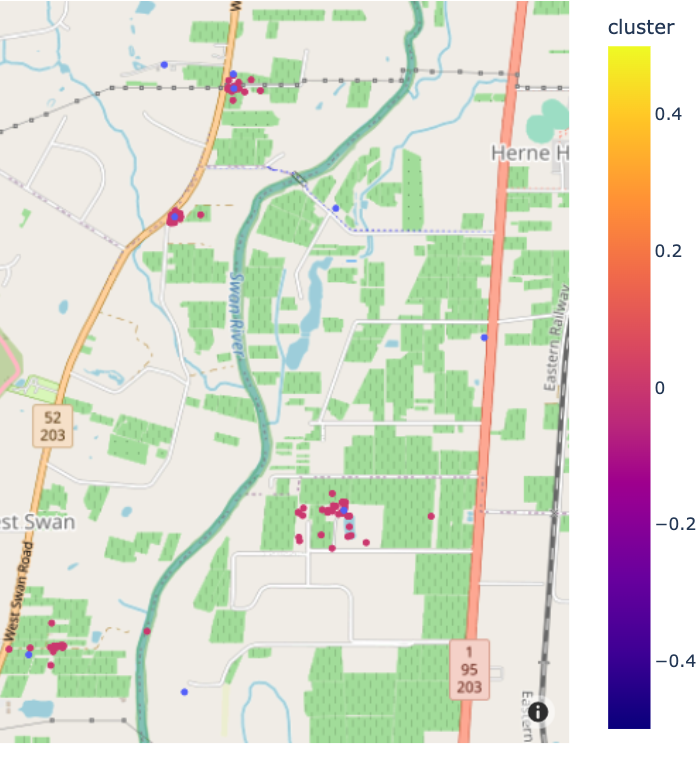
\includegraphics[width=\textwidth]{gestalt_dbscan_e1000.png}
%\caption{\small In worst-case settings where $\epsilon=1000$ (too large), it groups all objects into a single cluster and incorrectly assigns to the central location of the region}
%\label{fig:kmeans_worst}
%\hfill
%\end{subfigure}

%\caption{\textbf{DBSCAN Performance.} DBSCAN performs suboptimally when locations are close together and when $\epsilon$ is too small or too large}

%\label{fig:dbscan_experiments}
%\end{figure*}

%Discarding objects is problematic as it degrades the recall of objects that are distant from other objects. The experiments indicate that when $\epsilon$ values are small, more of the data is regarded as 'noise' and disregarded by the clustering algorithm. With $\epsilon=10m$, it forms 6 clusters, splitting \textit{Oakover Grounds} in half and discarding 12 objects of the ~150 as noise. Conversely, as $\epsilon$ increases, clusters rapidly begin to merge. Despite being distinct locations, the location merging problem is evident in the Winery Dataset when \textit{Ugly Duckling Wines} and \textit{Little River Winery and Cafe} combine. The worst case, where $\epsilon$ is set too large, merges all objects into a single, average location. The worst-case performance of DBSCAN matches the worst-case performance of K-Means with all objects belonging to the \textit{Sitealla} winery. 

\begin{table}[h!]
	\begin{center}
		\begin{tabular}{ |c|c|c|c|c| } 
			\hline
			Algorithm & Variant & Num Clusters & Accuracy \\
			\hline
			\multirow{3}{4em}{K-Means} & $K=1$ & 1 & 0/146 \\ 
			& $K=6$ & 6 & 146/146 \\ 
			& $K=31$ & 31 & 141/146 \\ 
			\hline
			\multirow{3}{4em}{DBSCAN} & $\epsilon=10m$, $N=3$ & 7 (+ 12 'noise') & 134/146 \\ 
			& $\epsilon=100m$, $N=3$ & 7 (+ 0 'noise') & 126/146 \\ 
			& $\epsilon=1000m$, $N=3$ & 1 (+ 0 'noise') & 0/146 \\ 
			\hline
		\end{tabular}
		\label{table:clustering}
		\caption{K-Means with perfect information performs best. DBSCAN handles dense inter-location clusters and variance in intra-object cluster density poorly}
	\end{center}
\end{table}

\subsection{Error Analysis}
Examining the errors reveals the following insights about each clustering technique. 

\textbf{When K-Means clusters incorrectly, labels are still correct.} When $K$ exceeds the number of clusters, it fragments the actual clusters. 
However, in ideal conditions like the Wineries Dataset, where locations are separated, the centroids of these cluster fragments are still closest to the correct location. 
As a consequence, they are correctly labelled despite being incorrectly clustered. We expect the accuracy will drop when locations are more densely packed. However, when we aim to process all objects and locations in a region concurrently, the number of clusters will likely approach the number of locations, and the issue will be less pronounced. 

\textbf{DBSCAN excludes outlying examples.} To prevent all locations in a region from being merged, a small $\epsilon$ is better. However, a small epsilon increases the number of points determined to be 'noise' and hence are not added to any cluster or provided with a label. 
The failure of DBSCAN to achieve 100\% recall of objects is problematic, as \textit{GESTALT} needs the maximal number of objects to be associated with candidate locations. Making $\epsilon$ larger, however, results in locations merging. As discussed in section \ref{section:implementation}, the DVBSCAN algorithm is a promising approach that will improve the ability to use a larger $\epsilon$ to improve recall without merging adjacent clusters. 

\subsection{Summary of Experimental Results}. 
The experiments reveal that small changes in the parameters of both K-Means and DBSCAN dramatically impact the output. K-Means performed the best under optimal conditions and better than DBSCAN under 'realistic' conditions. 
However, in datasets where locations have a higher density in the region, the benefit is expected to level, and so experimentation with an algorithm that can accept as a parameter the list of locations to use as clustering centroids seeks to overcome this issue in dense localities. 
DVBSCAN is the most promising avenue for implementing the improved ownership assignment. 
